\section{Ansys 算例与接口验证}
\label{chapter:09}

% block-id: 09.ansys.p1
\hypertarget{09.ansys.p1}{}
七股二维端口短测采用 704 单元，包含两个电压基解和第三次实际 ±20 A 场解。公共端电压、逐股复电流与独立功率为这一网格提供场路一致性检查，电流结果见 图~\ref{fig:ansys_seven_current}。其验证范围为单档网格；后续固定网格与精度尝试尚未形成完整三档验收，原生三维 J 表达式探针也未取得可接受的物理解。

% block-id: 09.ansys.p2
\hypertarget{09.ansys.p2}{}
图~\ref{fig:ansys_limits} 汇总已核查的 Ansys Student v252 能力：二维最多 2000 个三角形，三维最多 64000 个体单元和 8000 个面单元，计算最多使用 4 核。接口、许可规模和数值精度分别限制可执行的验证。实际端接、曲线 STL 与足铜大束研究需要与目标几何相匹配的许可和网格能力，并完成相应敏感性与功率检查。

% block-id: 09.figure.ansys_seven_current
\hypertarget{09.figure.ansys_seven_current}{}
\begin{figure}[!htbp]
\centering
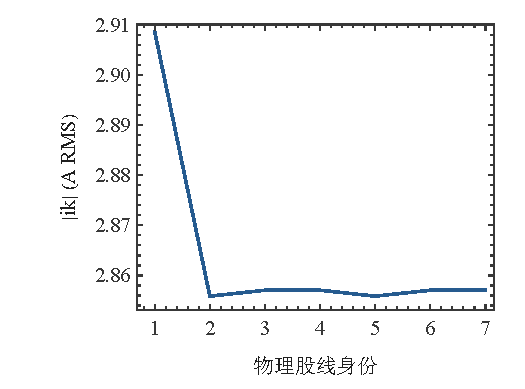
\includegraphics[width=\linewidth,height=.72\textheight,keepaspectratio]{../../assets/zh-CN/ansys_seven_current.pdf}
\caption{Ansys 七股二维复电流。 704 单元有效端口短测给出逐股幅值与相位。 电流采用实际 ±20 A 场解的端口记录。幅值与相位对应同一七股编号。}
\label{fig:ansys_seven_current}
\end{figure}

% block-id: 09.figure.ansys_limits
\hypertarget{09.figure.ansys_limits}{}
\begin{figure}[!htbp]
\centering
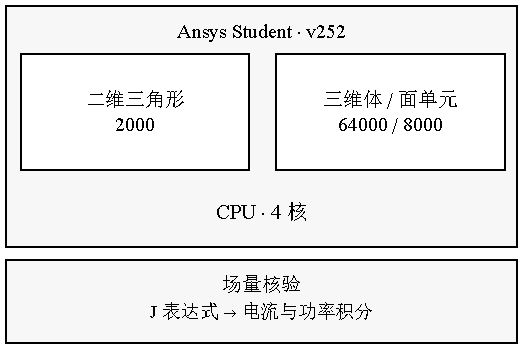
\includegraphics[width=\linewidth,height=.72\textheight,keepaspectratio]{../../assets/zh-CN/ansys_limits.pdf}
\caption{Ansys Student 能力与接口诊断。 Ansys Student v252 的许可规模及场量检查入口。二维上限为 2000 个三角形，三维上限为 64000 个体单元与 8000 个面单元，计算使用至多四核。许可边界来自 rc.1 保存记录，图件来源核对日期为 2026-10-15。}
\label{fig:ansys_limits}
\end{figure}

% block-id: 09.ansys.rc2
\hypertarget{09.ansys.rc2}{}
rc.2 进一步完成了通过 PyAEDT-MCP 的二维 Maxwell 建模、求解和工程回读，并保留任务取消及关联重启记录。与 Wolfram 的七股直束比较对齐截面、材料、频率、回流和总电流约束，逐股复电流相对 L2 差异为 0.0106814\%，束内 Rac 相对差异为 0.00132823\%。该比较使用独立网格，Maxwell 仅运行一次自适应求解，空间和边界收敛尚待检查。其成功说明对应二维端口链路已贯通；三维接口及足铜换位结构需要各自的场解与验收。\cite{PYAEDTMCP,PYAEDT}
